%!TEX root = ../main.tex

\chapter{Mlem Theory medicine}

\section{Inspiration in medicine}
The problem of reconstructing 3D positions of sources of ionizing radiation has been studied in depth in the field of medical imagining.
To give an example: one possible application of such methods is a cancer diagnostics.
A small amount of radioactive substance (called tracer) is injected into the patient's vein.
The tracer is absorbed by different parts of the body in varying amounts, which can show areas with abnormal metabolic activity, which is usually the case for cancer cells.
The detection of emitted particles and 3D reconstruction of their sources will allow the doctors to find the location of the tumor in the patient's body.

There are numerous methods used in medical imagining. 
Two main approaches are following: \ac{PET} and \ac{SPECT}.
\ac{PET} imagining typically use a gamma emitting radioisotope as a tracer.  
The method is based on positron emission. 
The emitted positron interacts with electron in the patients body and both particles vanish in a burst of energy. 
This energy comes in a form of two gamma rays, that goes into a opposite directions.
Detection of these two gamma rays (measured by the camera at the same time) allows us to reconstruct 3D image of the patient's body.
In \ac{SPECT}, single gamma ray is produced. 
The reconstructed image is computed from gamma rays detected by the camera.
Since only one gamma-ray is emmited (unlike in \ac{PET}), high number of measurements is needed for accute reconstruction.
Medical \ac{SPECT} imagining cameras typically use collimators to get some information about direction of incoming gamma ray.
Collimators restricts the set of possible directions from which the gamma ray may enter the detector (and be detected), therefore they can improve accuracy of the detection.

Another type of sensor (that can be used in \ac{SPECT} imagining) is a Compton camera.
The biggest benefit of compton camera is that it provides information about the direction of detected incoming gamma ray without the use of collimator.
The nuclear medicine reconstruction method for compton camera measurements that served as inspiration for for this thesis is called \ac{LM-MLEM}.

\section{Maximum likelihood expectation maximization}



\cite{1982_shepp_vardi_MLEM} \cite{EM} \cite{wilderman}

\subsection{Maximum likelihood estimation}
\ac{MLE} is a classical approach in machine learning.
It is used to estimate the parameters of a probability distribution based on observed data. 
The goal of \ac{MLE} is to find the parameter values that make the observed data most probable under the assumed probability distribution.
This is done by calculating the likelihood function, which is the probability of the observed data given a set of parameter values.
Likelihood can be defined as 
\begin{equation}
  likelihood = p(\ \mathrm{observations } \  \boldsymbol{O} | \ \mathrm{hidden \ parameters\ } \Phi ).
  \label{eq:likelihood}
\end{equation}
We want to maximize this expression with respect to the hidden parameters.
In other words, we want to find such parameters so that they fit our observations in the best possible way.

\section{Algorithm formulation}
Let's divide the area of possible sources of radiation into $J$ discrete bins (indexed with $j$, where $j = 1 \dotsc J$).
Each discrete bin is represented by its center position.
Suppose we have measurements divided into $I$ discrete bins indexed with $i$, $i = 1 \dotsc I$.
The vector $\mathbf{Y}$ with elements $y_{i}, i \in (1, \dots I)$ denotes the number of particles detected in the corresponding bin $i$.
Let's define matrix $\mathbf{T}$ ($\mathbf{T} \in \mathbb{R}^{I \times J}$), where each position in the matrix is defined as

\begin{equation}
  t_{ij} =  P(\textrm{detected in } i | \textrm{emitted from } j).
\end{equation}

In other words, $t_{ij}$ represents a probability that we observe observation $i$ given the fact that the radioactive particle was emitted from position $j$.

Let's assume that the number of photons emitted from one position $j$ is a discrete random variable that follows a Poisson distribution with expected value $\lambda_{j}$.
Our goal is to estimate $\mathbf{\Lambda}$, which has elements $\lambda_{j}$, each corresponding to the expected number of photons emitted from the position $j$.

The likelihood of measuring $y_{i}$ particles in the measurement bin $i$ w.r.t. $\mathbf{\Lambda}$ can be expressed as (Poisson distribution):
\begin{equation}
  p(y_{i} |\mu_{i} ) = e^{-\mu_{i}} \frac{\mu_{i}^{y_i}}{y_{i}!},
\end{equation}
where $\mu_{i} = \sum_{j} t_{ij}\lambda_{j}$ denotes the average number of events measured in bin $i$.

The likelihood of all the measurements is
\begin{equation}  
  p(\mathbf{Y} | \mathbf{T\Lambda} ) = \prod_{i} e^{-\mu_{i}} \frac{\mu_{i}^{y_i}}{y_{i}!}.
\end{equation}

After taking its logarithm, we have the following:

\begin{equation}  
  \mathrm{log}\ p(\mathbf{Y} | \mathbf{T\Lambda} ) = \sum_{i}\left ( -\sum_{j} t_{ij}\lambda_{j} + y_{i} \mathrm{log}(\sum_{j} t_{ij}\lambda_{j})  - \mathrm{log}(y_{i}!) \right ).
  \label{eq:likelihood1}
\end{equation}
However, equation \ref{eq:likelihood1} doesn't give an answer to our question - how to determine $\mathbf{\Lambda}$. The solution is to use an iterative \ac{EM} algorithm.

The \ac{EM} algorithm was originally proposed by \cite{EM}. 

\section{differences}
Such medical application typically requires high resolution of the reconstructed image.
The distances between the source and detector are small (tens of centimeters), number of measured events is high (tens of thousands and more).
The reconstruction process is typically performed offline (all measurements are collected first and then the algorithms process the data), since there is no need for online estimation and the processing of measured data might take non-negligible time.
The domain of multirobotic radiation mapping has multiple differences compared to the medical field.
The distance between source and detector is much higher (tens of meters).
The \ac{UAV}s have limited payload (hence the detector carried on board must be light and compact).
It results in the fact that the number of measurements is much lower (hundreds-thousands detected compton events).
Moreover, we would like to reconstruct the sources of ionizing radiation in real time.
Despite all of these differences, the aim of this work is to adapt such algorithms to our problem.

\chapter{Methods}
The \ac{MLEM} algorithm described previously serves as an inspiration for the mapping method described in this chapter.
Despite all the differences between the medical and multirobotic domain, the \ac{MLEM} algorithm was chosen for several reasons.
First of all, the nature of the measurements (compton cones) is the same as in the medical algorithms.
Secondly, the classical method of maximization of likelihood of measured data seems to be good choice for the given problem.
It can take into account factors influencing the measurements (such as air attenuation, properties of the detector and radioactive emission) in the probabilistic way.
Lastly, the estimation of sensitivity of detection (how likely the particles from given position were measured) can be beneficial, 
because it can provide information of how much the \ac{UAV}s already explored the area of interest and where to fly to possibly detect undetected sources.



\section{Setup}
Figure \ref{fig:discretization} shows the discretization of the area of interest.
The area where possible sources of ionizing radiation might be located is divided into $J$ discrete bins, each of them is approximated by its center position and indexed as $j$.
The individual measurements (compton cones) are indexed with $i$, $i \in 1, \dots , I$, where $I$ is the total number of measurements collected during the experiment.
Let's denote $\mathbf{\Lambda}$ ($\mathbf{\Lambda} = \begin{bmatrix}\lambda_{0} & \lambda_{1} & \dots & \lambda_{J}\end{bmatrix}$) as the vector of hidden parameters we would like to estimate.
As described in the previous chapter, $\lambda_{j}$ represents the expected number of particles emitted from the corresponding map position $j$ in the unit time interval.

\begin{figure}[!h]
  \centering

  \subfloat[area of interest] {
    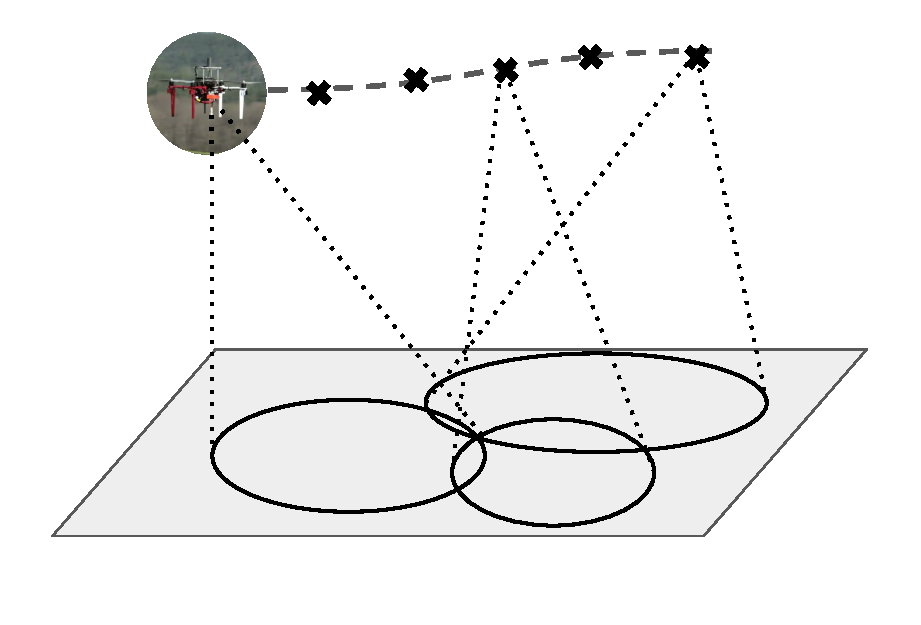
\includegraphics[width=0.32\textwidth]{./fig/photos/dis1.eps}
    \label{fig:dis1}
  }
  \subfloat[discretization] {
    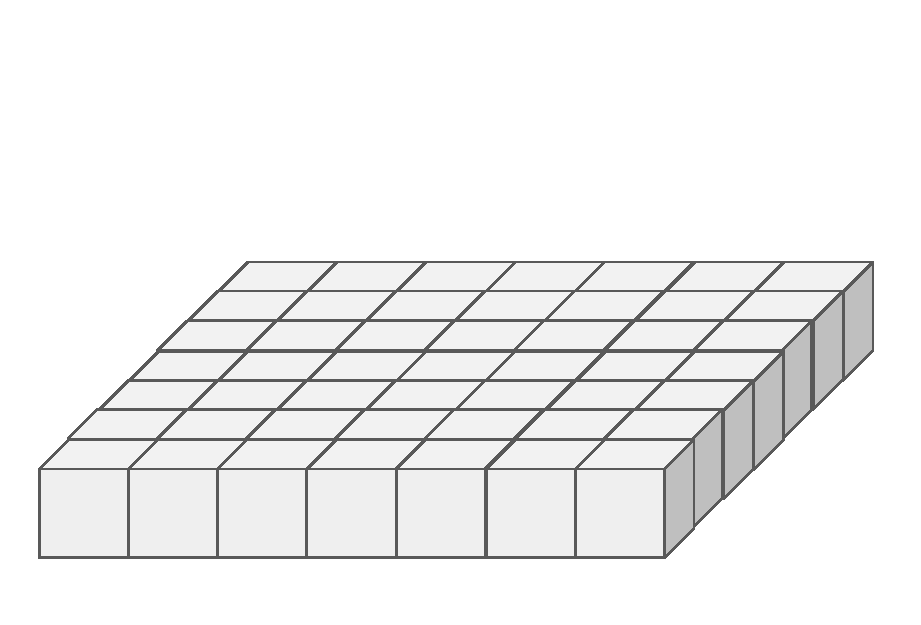
\includegraphics[width=0.32\textwidth]{./fig/photos/dis2.eps}
    \label{fig:dis2}
  }
  \subfloat[hidden parameters $\Lambda$] {
    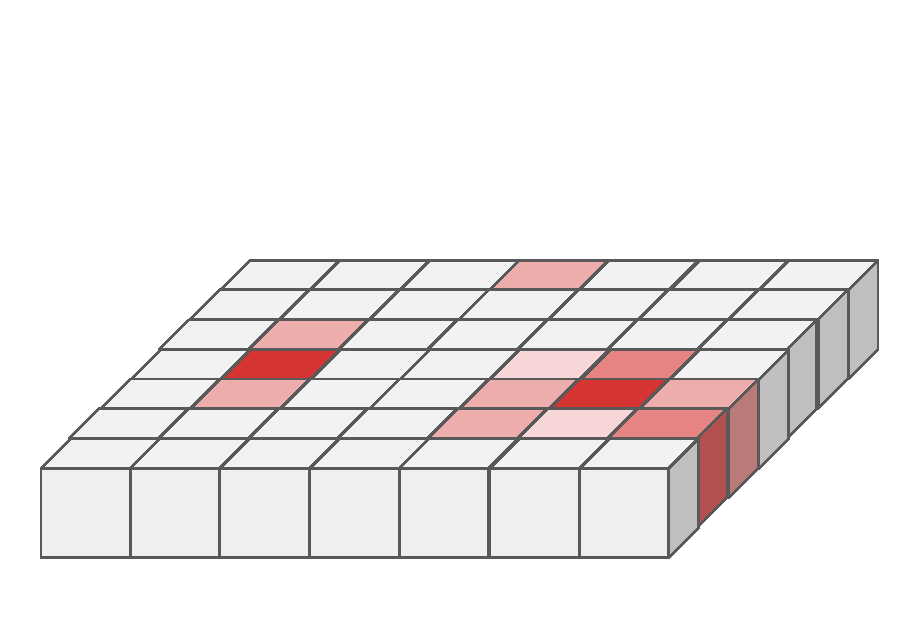
\includegraphics[width=0.32\textwidth]{./fig/photos/dis3.eps}
    \label{fig:dis3}
  }
  \caption{An illustration of algorithm setting}
  \label{fig:discretization}
\end{figure}

\section{MLEM}
The estimation process proceeds interatively using the \ac{LM-MLEM} algorithm:
\begin{equation}
  \hat{\lambda}_{j}^{[l]} = \frac{\hat{\lambda}_{j}^{[l-1]}}{s_{j}} \sum_{i \in I} \frac{t_{ij}}{\sum_{k} t_{ik} \hat{\lambda}_{k}^{[l-1]}},
  \label{eq:MLEM}
\end{equation}
where $l$ is the current iteration of the algorithm, $\lambda_{j}$ is the hidden parameter for each position $j$ we would like to estimate, $t_{ij}$ is the element of system matrix $\mathbf{T}$ and $s_{j}$ is the sensitivity of detection for the map position $j$.
The estimation of system matrix $\mathbf{T}$ and sensitivity of detection $\mathbf{S}$ is described in the following sections.


\section{Sensitivity of detection}
The probability of a photon emitted from a given position $j$ to be detected by the compton camera is called sensitivity of detection.
It can be expressed using conditional probability as 
\begin{equation}
  s_{j} =  P(\textrm{detected by the sensor}\ | \textrm{emitted from } j).
\end{equation}

A series of random occurrences should happen for a photon to be detected by the compton camera.
First of all, the photon must be emitted from position $j$ towards the sensor surface (emitted under the solid angle subtended by the visible camera surface at the position of the source), not being absorbed by the air along the way.
Then the photon should interact with the matter of the sensor in form of compton scattering.
The angle under which it scatters is described by the Klein-Nisnina cross section.
The scattered photon then must be absorbed by the camera in form of a photoelectric effect.
This model is simplified, because other random occurrences might happen - for example the photon might undergo \ac{CS} twice in a row, the sensor might not detect the interations properly, etc.
However, we will stick to the proposed simplified model with particles undergoing \ac{CS} and then \ac{PE} interactions consecutively.

The literature describes several analytical models for computing sensitivity of the detection. 
For example \cite{wilderman2001} proposed sensitivity model for multi-layer compton cameras in the close distance to the source.
\cite{maxim2016} proposed simplified model for comptom-cameras with negligible size compared to the distance from the source.
However, these models are not suitable for the problem tackled in this thesis.
The multi-layer compton camera has different properties then single-layer sensor \ac{pix}.
Multi-layer compton cameras are typically measuring only particles coming from certain directions (from the front side of the camera, perpendicular to its layers).
On the other hand, the \ac{pix} sensor used in this project can potentially measure particles coming from all directions.
The sensitivity of the sensor w.r.t. different directions of the incoming particle is unknown and present a scientific question, that needs to be answered to make the \ac{LM-MLEM} working. 

Another option presented in literature is evaluation of sensitivity using the Monte-carlo simulation.
This approach has multiple advantages: it is not necessary to describe all random occurrences inside the detector by a single expression (which might take non-negligible computation time when evaluating big number of map positions during the experiment).
Monte-carlo simulation can be precomputed in advance and the data can be stored in some data structure that allows fast access to the data, shortening the computation time.

In our case, the position of the detector is not static. 
The \ac{UAV}s carrying the compton camera are dynamically moving through the environment, with varying speed, position and orientation.
Therefore, the positions of the \ac{UAV}s are sampled in time from \ac{UAV}s trajectories and denoted as $v$, where $v \in (0, \dots , V)$ and $V$ is the total number of viewpoints generated by all \ac{UAV}s during the experiment.
The sensitivity of detection is evaluated for each $jv$ pair. 

\begin{figure}[!h]
  \centering
    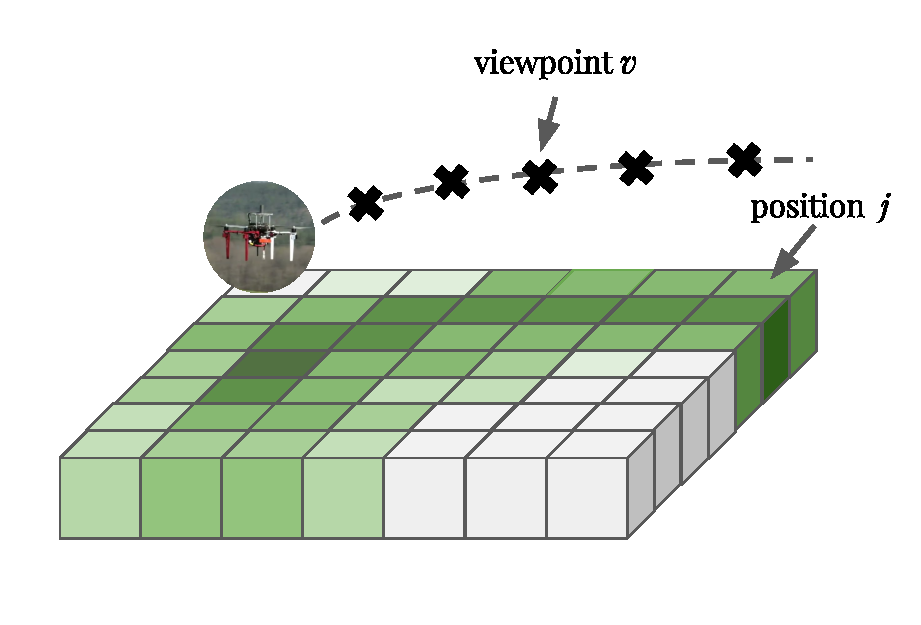
\includegraphics[width=0.6\textwidth]{./fig/photos/sen.eps}
    \label{fig:sen_illustration}
  \caption{An illustration of sensitivity computation. Sensitivity describes probability that particle emitted at given position is measured by the compton cameras onboard the \ac{UAV}s. In other words, it describes how well explored is given map position during the experiment. The trajectory of the \ac{UAV} is sampled into viewpoints denoted as $v$.}
\end{figure}

\subsection{Probabilistic description}

The series of random occurrences for a photon emitted at position $J$ leading to the detection by the compton camera at position $v$ can be described as follows:
\begin{equation}
  s_{jv} =  (p_{solid\ angle})(1-p_{air})(p_{compton})(p_{absorbtion}),
\end{equation}

where $p_{solid\ angle}$ is the probability that photon is emitted towards the solid angle of the detector, $p_{air}$ is the probability that photon is absorbed by the air along the way from emission towards the sensor, $p_{compton}$ is probability that compton scattering occurs and $p_{absorbtion}$ denotes that scattered photon is absorbed by the detector and measured.
We want to approximate the $(p_{solid\ angle})$, $(p_{compton})$ and $(p_{absorbtion})$ using a Monte-carlo simulation.

\subsection{Monte carlo simulation}
The idea of Monte-carlo simulation is simple:
instead of deriving analytical expression,
which might be complicated given the nature of the \ac{pix} detector (where all interactions are happening in a single block of matter and probabilities of \ac{CS} or \ac{PE} depend on the length of the ray segment inside the sensor) and time-comsuming for online computations during the experiment,
we will place simulated sources at certain position and compute how many particles produced compton cones in the simulated sensor.
The realistic compton camera simulator described \cite{baca2019timepix} was used as a template and adapted for this particular application.


%Figure \ref{fig:polar} shows the polar coordinate system, where angles $\theta$ and $\phi$ determines the relative position of the source with respect to the compton camera.

Position of each simulated source is parametrized by its polar coordinates (angles $\theta$ , $\phi$ and distance $d$), as shown in figure \ref{fig:polar}.
Each simulated source emits $N$ particles (in all directions).
Since the compton camera is a symmetrical object, only $\frac{1}{8}$ of the elementary sphere around the detector needs to be simulated.
Figure \ref{fig:sources_loc} shows the positions of simulated sources and figure \ref{fig:sampling} presents their positions in the angle space.
We compute the probability of producing a compton cone for particle emitted by a source at relative position given by polar coordinates ($\theta, \phi, d$) as
\begin{equation}
  p(\mathrm{cone\ detection})_{(\theta, \phi, d)} = \frac{C_{(\theta, \phi, d)}}{N},
\end{equation} 
where $C_{(\theta, \phi, d)}$ is the number of particles that undergone \ac{CS} and \ac{PE} consecutively inside the compton camera (therefore can be detected), $N$ is the number of all particles emitted at source position $(\theta, \phi, d)$. 
Number of emitted particles is $N = 1\mathrm{e}11$, the distance $d$ is set to $d = \SI{1}\meter$.
The simulation process is described in algorithm \ref{alg:monte}. 
The results of the simulation are stored in a lookup table:
\begin{equation}
  \mathrm{lookup\_table}(\theta_{k}, \phi_{k}) = p(\mathrm{cone\ detection})_{(\theta_{k}, \phi_{k}, d = \SI{1}\meter)}. 
\end{equation}
It is a data structure that allows fast readout of the stored data.
For arbitrary query ($\theta, \phi$) it finds the closest key pair ($\theta_{k}, \phi_{k}$) in the angle space and returns its value.

%multifigure montecarlo
\begin{figure}[!h]% %%{
  \centering

  \subfloat[\centering Polar coordinates] {
    \centering
    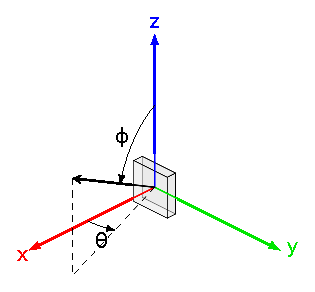
\includegraphics[width=0.3\textwidth]{./fig/photos/axes.eps}
    \label{fig:polar}
  }
  \subfloat[\centering Locations of the simulated sources] {
    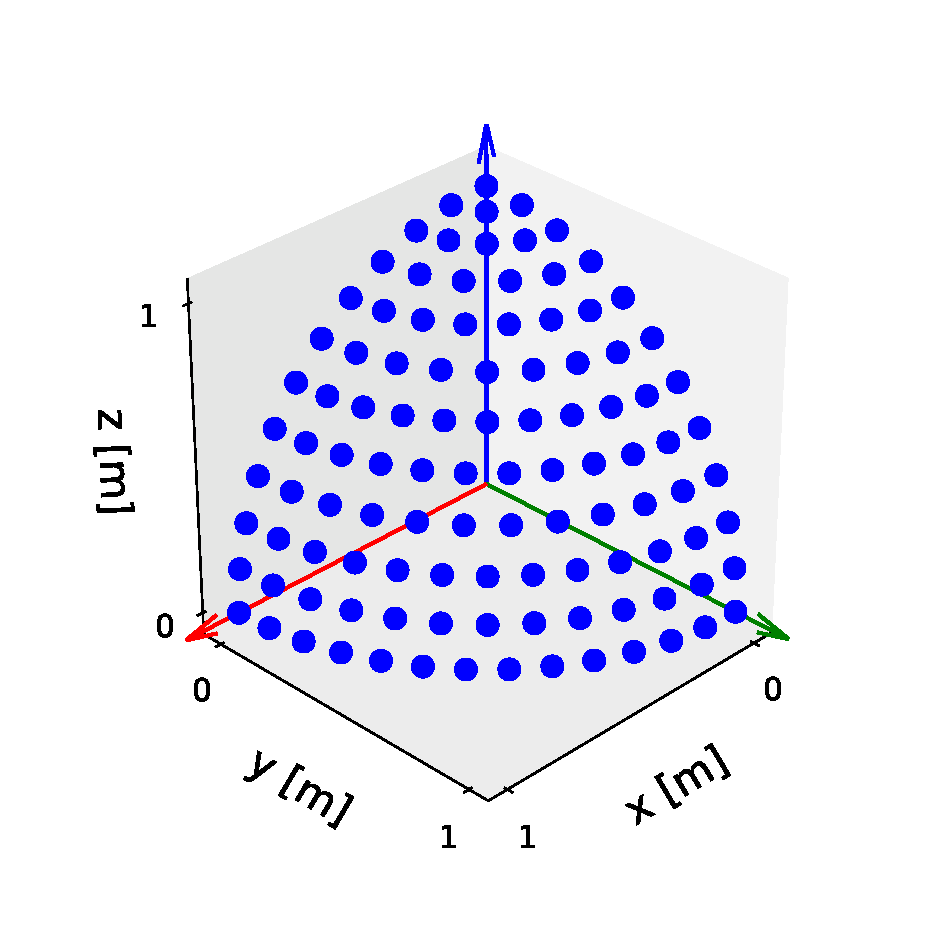
\includegraphics[width=0.33\textwidth]{./fig/photos/mc_sources.eps}
    \label{fig:sources_loc}
  }
  \subfloat[\centering Sampling of the $\frac{1}{8}$ of the unit sphere in the angle space] {
    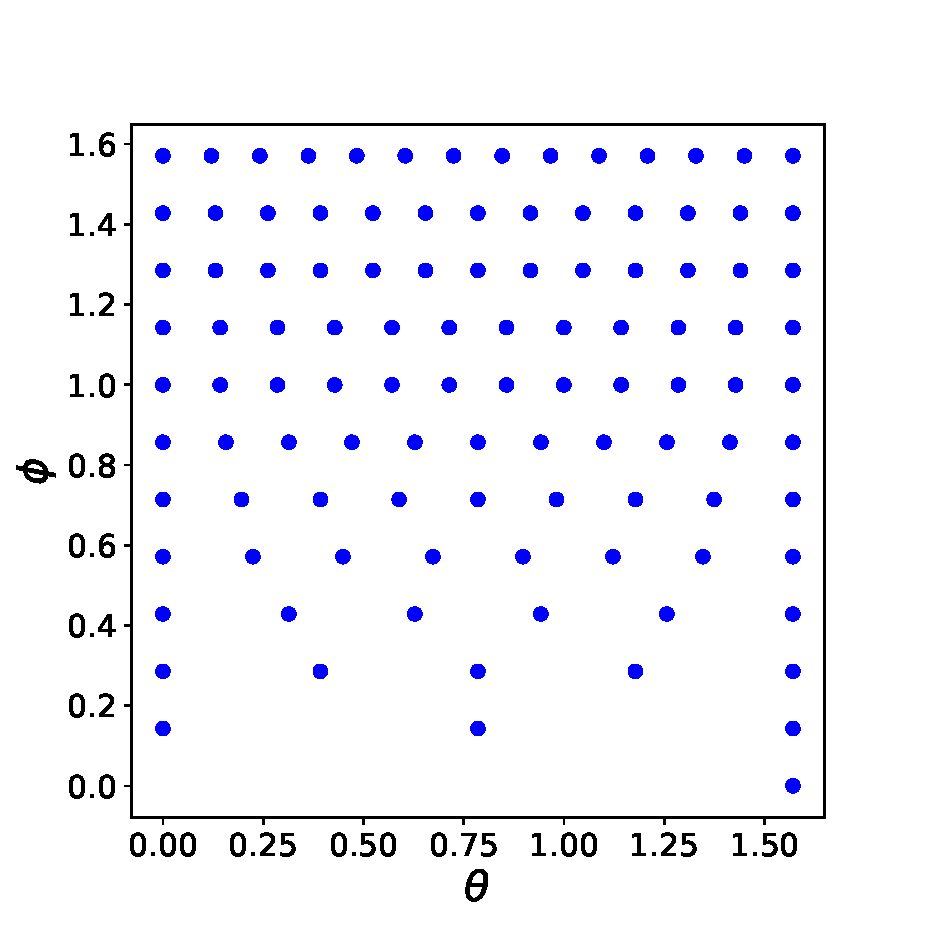
\includegraphics[width=0.33\textwidth]{./fig/photos/mc_angle_space.eps}
    \label{fig:sampling}
  }
  \caption{}
  \label{fig:mc_multi}
\end{figure}% %%}

%%%%%%%%%%% ALGORITHM %%%%%%%%%%%%%%%%%% %%{
%%%%%%%%%%%%%%%%%%%%%%%%%%%%%%%%%%%%%%%%%%%
\begin{algorithm}[h!]
\caption{Monte-carlo simulation}\label{alg:cap}
\begin{algorithmic}
\Function {create\_lookup\_table}{$N$}
  \For {$\theta \in (0, \dots ,\frac{\pi}{2})$}
    \For {$\phi \in (0, \dots , \frac{\pi}{2})$}
      \State $\mathrm{lookup\_table}(\theta, \phi) \gets \Call{compute\_probability}{\theta, \phi, N}$
    \EndFor
  \EndFor
\EndFunction
\Statex
\Function {compute\_probability}{$\theta, \phi, N$}
\State $C \gets 0$
\State $A \gets N\frac{\Omega_{\theta, \phi}}{4 \pi}$ \Comment{how many of $N$ particles hits the sensor}
\State $a \gets 0$
\While {$a<A$} 
  \If {\Call{is\_cone\_measured}{$\theta, \phi$}} \Comment{Compton cone measured}
  \State $C \gets C + 1 $ 
  \EndIf
  \State $a \gets a + 1$
\EndWhile
  \State \Return $C/N$ 
  \EndFunction
\Statex
  \Function{is\_cone\_measured}{$\theta,\phi$}
  \State $ray \gets \Call{sample\_sensor\_surface}{\theta,\phi}$ \Comment{ray inside the sensor after hitting its surface}
  \If{\Call{is\_compton\_scattering}{$ray, E_{0}$}} \Comment{sample if \ac{CS} occured}
  \State $new\_ray, E_{1} \gets \Call{compton\_scattering}{ray, E_{0}}$ \Comment{Sample Klein-Nishina formula}
  \Else{}
    \State \Return False \Comment{No compton scattering occured}
  \EndIf
  \If{\Call{is\_photoelectric\_effect}{$new\_ray, E_{1}$}} \Comment{Sample if \ac{PE} occured} 
    \State \Return True
  \Else{}
    \State \Return False
  \EndIf
\EndFunction
\end{algorithmic}
  \label{alg:monte}
  \caption{Monte-carlo simulation}
\end{algorithm}

%%%%%%%%%%%%%%%%%%%%%%%%%%%%%%%%%%%%%%%%%%%% %%}

\section{Sensitivity matrix}
The sensitivity of detection by the sensor placed at sampled position $v$ for map position $j$ is computed as:

\begin{equation}
  s_{jv} = \underset{(1-p_{air})}{\underbrace{e^{-((\mu/\rho) d_{jv})} }} \underset{(p_{solid\ angle})\\(p_{compton})\\(p_{absorbtion})} {\underbrace{\frac{\mathrm{lookup\_table}(\phi_{jv}, \theta_{jv})}{d^{2}_{jv}}}},  
  \label{eq:sjv}
\end{equation}
where $d_{jv}$ is the euclidean distance between map position $j$ and sensor position $v$, ($\mu/\rho$) is the total attenuation coefficient for air (based on \cite{nist}), ($\phi_{jv}, \theta_{jv}$) are polar coordinates determining the relative position of $v$ and the sensor. 
The term $\frac{1}{d^{2}_{jv}}$ in \ref{eq:sjv} ensures that the $p_{solid\ angle}$ (already contained in the $\mathrm{lookup\_table}$ for $d = \SI{1}\meter$) approximately holds even for distances other than $d = \SI{1}\meter$.

\subsection{Iterative formula}
The equation \ref{eq:sjv} presents the sensitivity computation for one viewpoint $v$. 
It is required to compute the sensitivity of detection online during the experiment for all the viewpoints from all \ac{UAV}s sampled so far. 
Therefore it is iteratively updated with the new sampled viewpoints (\ac{UAV} positions).
Let denote $\mathbf{S}^{[n]}$ the sensitivity matrix at update step $n$.
The initial value of $\mathbf{S}^{[0]}$ is set to $0$ ($s_{j}^{[0]} = 0 ,\forall s_{j}^{[0]} \in \mathbf{S}^{[0]}$).
Lets denote $V^{[n:n+1]}$ the set of viewpoints that were newly sampled after update step $n$ and needs to be processed. 

The sensitivity matrix $\mathbf{S}^{[n+1]}$ with elements $s_{j}^{[n+1]}$ is computed as follows:
\begin{equation}
  s_{j}^{[n+1]} = s_{j}^{[n]} + \sum_{v \in V^{[n:n+1]}} s_{jv} \Delta_{v}, 
  \label{eq:sen_iter}
\end{equation}
where the sum $\sum_{v \in V^{[n:n+1]}}$ iterates over all newly processed viewpoints, 
the term $\Delta_{v} = t_{v} - t_{v-1}$ expresses the time difference between current viewpoint $v$ sampled at time $t_{v}$ and its predecessor (previous viewpoint generated from the trajectory of the same \ac{UAV}) sampled at time $t_{v-1}$. 

This formulation of sensitivity has multiple advantages.
Firstly, the memory requirements for storing the matrix $\mathbf{S}$ remain the same during the whole experiment, the values $s_{j}$ are updated in place.
Secondly, the sensitivity is updated online as new sampled trajectories of the \ac{UAV} arrive, therefore the computation time scale well with increasing duration of the experiment.
Lastly, it takes into account the time difference between sampled viewpoints $\Delta_{v}$.

\section{System matrix}
The system matrix $\mathbf{T} \in \mathbb{R}^{I \times J}$ is defined as
\begin{equation}
t_{ij} =  P(\textrm{detected in } i | \textrm{emitted from } j).
\end{equation}
In other words, it says how likely the photon causing measurement $i$ came from the map position $j$.
The illustration of the system matrix is depicted in figure \ref{fig:sys_ilustration}, where the blue color represents $t_{ij}$ values of the individual cells. 
\begin{figure}[!h]
  \centering

    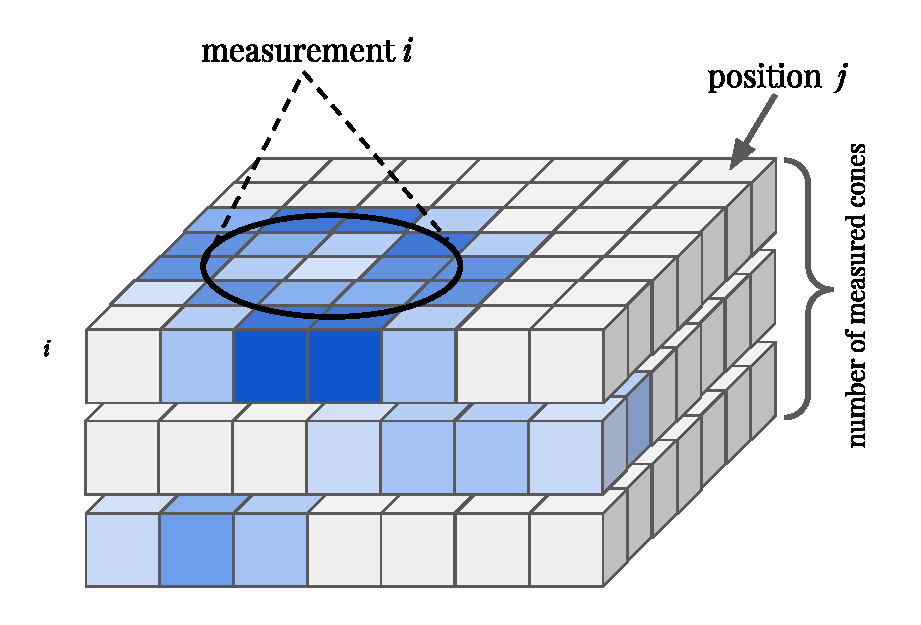
\includegraphics[width=0.48\textwidth]{./fig/photos/sys.eps}
  \caption{System matrix $\mathbf{T}$. The blue color represent the value of $t_{ij}$ in each cell.}
    \label{fig:sys_ilustration}
\end{figure}

The main question remains the same as for the sensitivity computation: how to evaluate the system matrix for given scenario and \ac{pix} sensor?

The measurement $i$ is composed of multiple components:
The first interaction (electron produced as a side product of \ac{CS}) at position $X_{1}$) with measured energy $E_{1}$ 
and the second interaction (absorbed electron at position $X_{2}$ inside the sensor with measured energy $E_{2}$.
The compton cone $i$ with scattering angle $\Theta$ is then reconstructed from these measurements using equation \ref{eq:theta}.



\subsection{Literature overview}

where 
\begin{itemize}
  \item $P_{1}$ is probability that photon is emmited
  \item $P_{2}$ is probability that photon is absorbed by the air
  \item $P_{3}$ is probability that photon reaches the detector
  \item $P_{4}$ is probablility that compton scattering occured
  \item $P_{5}$ is probability that photoelectric effect occured
\end{itemize}







\begin{equation}
  t_{ij} =  (1-p_{air})  K(\beta_{i},E_{0}) \frac{}{d^{2}_{ij}} h(\delta_{ij}, \phi)
\end{equation}


\begin{equation}
  t_{ij} =  p_{1}p_{2}p_{3}p_{4}p_{5}
\end{equation}

